\textbf{\textcolor{darkblue}{ JPA}}~

\section*{JPA}
\subsection*{Frage 1}
Was ist ein OR-Mapper und was versteht man unter „object relational impedance mismatch“?
\subsection*{Antwort}
OR-Mapper: Objekt-Relatonaler-Mapper (Abbildung von Datenbankschema auf Programmierschema),
Object relational impedance: Die Unverträglichkeit zwischen der objektorientierten Programmiersprache und einer relationalen Datenbank bei z. B. Vererbungen 
\subsection*{Frage 2}
Was sind die Vorteile von JPA gegenüber DAO?
\subsection*{Antwort}
\begin{itemize}
	\item SQL-Abfragen müssen nicht vom Programmierer geschrieben werden (Automatische Generierung von SQL-Abfragen)
	\item Unabhängigkeit zur Datenbank
	\item Standardisierte Schnittstelle zur Datenbank
	\item Objekte werden durch Funktionsaufrufe persistiert
\end{itemize}

\subsection*{Frage 3}
Welche Komponenten von JPA gibt es und wie arbeiten sie zusammen?
\subsection*{Antwort}
\begin{itemize}
	\item Enitity-Manager: zentrale Programmierschnittstelle zur Datenbanksteuerung
	\item Persistenz-Kontext: Zwischenspeicher des Entity-Managers
	\item Life Cycle von Objekten:
\end{itemize}
\subsection*{Frage 4}
Was sind die Stärken und Schwächen von OR-Mappern
\subsection*{Antwort}
\begin{figure}
		\centering
		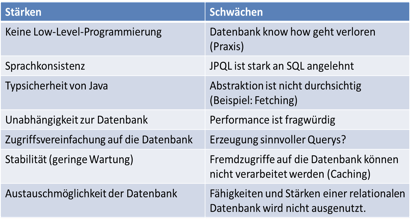
\includegraphics[width=0.7\linewidth]{screenshot001}
		\caption{}
		\label{fig:screenshot001}
	\end{figure}
\subsection*{Frage 5}
Welche Grundvoraussetzungen müssen erfüllt sein, sodass ein Java-Objekt als JPA Entität erkannt wird?
\subsection*{Antwort}
\begin{itemize}
	\item muss class oder abstract class sein
	\item default konstruktor
	\item Interface implementieren java.io.Serializable
	\item Keine Kennzeichnung der JPA-Entities mit final
	\item Vorhandensein von Primärschlüssel für die gemappte Datenbanktabelle 
	\item @Entity @Id
\end{itemize}
\subsection*{Frage 6}
Was ist der Unterschied zwischen einer uni- und einer bidirektionalen Assoziation?
\subsection*{Antwort}
Unidirektional: Wenn Objekte einer Seite (Klasse A) auf zugeordnete Objekte der anderen Seite (Klasse B) zugreifen kann.  Datenübertragung in eine Richtung
Bidirektional: Wenn auch der umgekehrte Fall gilt; also, dass von Objekten der Klasse B auch auf Objekte der Klasse A zugegriffen werden kann  Datenübertragung in beide Richtungen

\subsection*{Frage 7}
Was sind die grundlegenden Funktionen vom Entity-Manager?
\subsection*{Antwort}
\begin{figure}
	\centering
	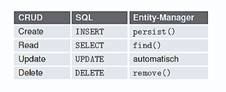
\includegraphics[width=0.7\linewidth]{screenshot002}
	\caption{}
	\label{fig:screenshot002}
\end{figure}

\subsection*{Frage 8}
Welchen Nachteil von JPQL gleicht die Criteria API aus?
\subsection*{Antwort}
JPQL-Anfragen basieren zum großen Teil auf Strings. Dadurch kann die Anfrage nicht auf syntaktische Korrektheit überprüft werden. Etwaige Tippfehler werden erst zur Laufzeit bemerkt und lösen Laufzeitfehler aus.
Die Criteria API verwendet ein komplexes Klassenmodell um Strings soweit wie möglich aus der Anfrage-Erstellung herauszuhalten. Dafür hat der Programmierer keine Kontrolle mehr über die Performanz der erzeugten SQL-Abfragen.